\subsubsection{Adams-Bashforth}

Table \ref{tab:oscillation_errors_ab} summarizes the Adams-Bashforth error analysis. As expected, the Adams-Bashforth 1 step solution, that reverts back to the explicit forward Euler one, is unstable for all the $\Delta t$ exercised.

The expected observed orders of accuracy for the Adams-Bashforth solvers using 2, 3 and 4 time steps tend to 1.5, 2.5 and 3.5 that are in agreement with the expected formal order of 2, 3 and 4, respectively. Comparing the errors of the finest time resolution, i.e. $\Delta t=100$, we find that the L2 norm decreases of the 2 orders of magnitude as the solver's accuracy increases by 1 order. This also means that fixing a tolerance on the errors, the higher is the solver's accuracy the larger is the time resolution available. As an example, assuming that admissible errors are of $O(10^{-2})$ with the 4-steps solver we can use $\Delta t=625$ performing $N_s=t_final/625$ numerical integration steps, whereas using a 3-steps solvers we must adopt $\Delta t=100$ performing $6.25 \times N_s$ numerical integration steps instead of $N_s$. Considering that the computational costs is only slightly affected by the number of previous time steps considered\footnote{Recalling equation \ref{eq:AB} one can observe that there is only one new evaluation of the residuals function $R$ independently of the previous time steps considered. Thus, the computational costs is affected only by the increasing number of residuals summations, the costs of which are typically negligible with respect the cost of $R$ evaluation.}, the accuracy order has strong impact on the overall numerical efficiency: to improve the numerical efficiency reducing the computational costs, the usage of high order Adams-Bashforth solvers with larger time steps should be preferred instead of low order solvers with smaller time steps.

\begin{table}[!ht]
  \centering
  \caption{Oscillation test: errors analysis of explicit Adams-Bashforth solvers}\label{tab:oscillation_errors_ab}
  \begin{subtable}[b]{0.40\textwidth}
    \centering
    \caption{1 step}\label{tab:oscillation-ab-1}
    \resizebox{1.00\textwidth}{!}{%
    \begin{tabular}{ccccc}
      \toprule
      {\sc Time Step} & {\sc Error X} & {\sc Error Y} & {\sc Order X} & {\sc Order Y} \\
      \hline
      5000.0          &  0.840E+10    &  0.706E+10    & /             & /             \\
      2500.0          &  0.503E+06    &  0.570E+06    & 14.03         & 13.60         \\
      1250.0          &  0.289E+04    &  0.272E+04    &  7.45         &  7.71         \\
       625.0          &  0.239E+03    &  0.232E+03    &  3.59         &  3.55         \\
       320.0          &  0.737E+02    &  0.722E+02    &  1.76         &  1.74         \\
       100.0          &  0.250E+02    &  0.247E+02    &  0.93         &  0.92         \\
      \bottomrule
    \end{tabular}}
  \end{subtable}\quad%
  \begin{subtable}[b]{0.40\textwidth}
    \centering
    \caption{2 steps}\label{tab:oscillation-ab-2}
    \resizebox{1.00\textwidth}{!}{%
    \begin{tabular}{ccccc}
      \toprule
      {\sc Time Step} & {\sc Error X} & {\sc Error Y} & {\sc Order X} & {\sc Order Y} \\
      \hline
      5000.0          &  0.596E+03    &  0.583E+03    & /             & /             \\
      2500.0          &  0.221E+02    &  0.218E+02    & 4.75          & 4.74          \\
      1250.0          &  0.764E+01    &  0.769E+01    & 1.53          & 1.50          \\
       625.0          &  0.265E+01    &  0.268E+01    & 1.53          & 1.52          \\
       320.0          &  0.968E+00    &  0.981E+00    & 1.51          & 1.50          \\
       100.0          &  0.169E+00    &  0.171E+00    & 1.50          & 1.50          \\
      \bottomrule
    \end{tabular}}
  \end{subtable}\\
  \begin{subtable}[b]{0.40\textwidth}
    \centering
    \caption{3 steps}\label{tab:oscillation-ab-3}
    \resizebox{1.00\textwidth}{!}{%
    \begin{tabular}{ccccc}
      \toprule
      {\sc Time Step} & {\sc Error X} & {\sc Error Y} & {\sc Order X} & {\sc Order Y} \\
      \hline
      5000.0          &  0.857E+01    &  0.854E+01    & /             & /             \\
      2500.0          &  0.391E+01    &  0.386E+01    & 1.13          & 1.14          \\
      1250.0          &  0.825E+00    &  0.814E+00    & 2.24          & 2.25          \\
       625.0          &  0.150E+00    &  0.148E+00    & 2.46          & 2.46          \\
       320.0          &  0.282E-01    &  0.278E-01    & 2.49          & 2.49          \\
       100.0          &  0.154E-02    &  0.152E-02    & 2.50          & 2.50          \\
      \bottomrule
    \end{tabular}}
  \end{subtable}\quad%
  \begin{subtable}[b]{0.40\textwidth}
    \centering
    \caption{4 steps}\label{tab:oscillation-ab-4}
    \resizebox{1.00\textwidth}{!}{%
    \begin{tabular}{ccccc}
      \toprule
      {\sc Time Step} & {\sc Error X} & {\sc Error Y} & {\sc Order X} & {\sc Order Y} \\
      \hline
      5000.0          &  0.128E+07    &  0.143E+07    & /             & /             \\
      2500.0          &  0.106E+01    &  0.107E+01    & 20.21         & 20.34         \\
      1250.0          &  0.967E-01    &  0.981E-01    &  3.45         &  3.45         \\
       625.0          &  0.859E-02    &  0.871E-02    &  3.49         &  3.49         \\
       320.0          &  0.827E-03    &  0.838E-03    &  3.50         &  3.50         \\
       100.0          &  0.141E-04    &  0.143E-04    &  3.50         &  3.50         \\
      \bottomrule
    \end{tabular}}
  \end{subtable}\\
\end{table}

Figure \ref{fig:results-oscillation-adams-bashforth} shows, for each solver exercised, the $X(t)$ and $Y(t)$ solution for $t \in [0, 10^6]$: the plots into the figure report a global overview of the solution for all the instants considered (left subplots) and a detailed zoom over the last instants of the integration (right subplots) for evaluating the numerical errors accumulation. For the sake of clarity, the strongly unstable solutions are omitted into the subplots concerning the final integration instants, namely the solutions for large $\Delta t$. Figure \ref{fig:results-oscillation-adams-bashforth} emphasizes the instability generation for some pairs steps number/$\Delta t$. The 2 and 4 steps solutions are instable for $\Delta t=5000 \rightarrow f*\Delta t=0.5$. On the contrary, the 3 steps solution is stable, but the amplitude is dumped and the solution vanishes as the integration proceeds. The 2 and 4 steps solutions show a phase error that decreases as the time resolution increases, whereas 3 steps solution has null phase error.

\begin{figure}[!ht]
  \centering
  \begin{subfigure}[b]{0.45\textwidth}
    \centering
    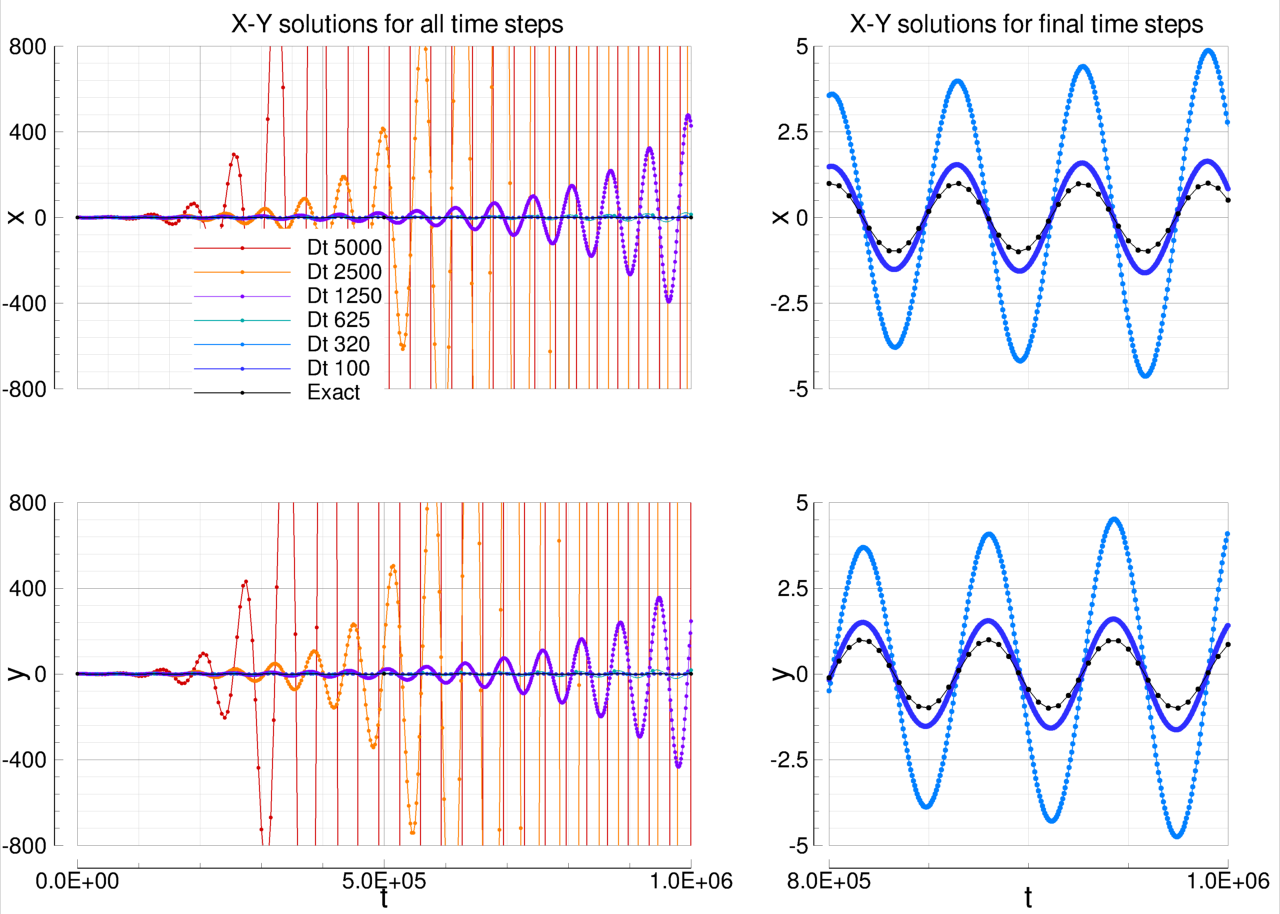
\includegraphics[width=1.00\textwidth]{errors-analysis/oscillation/errors_analysis-oscillation-adams-bashforth-1.png}
    \caption{1 step}\label{fig:results-oscillation-adams-bashforth-1}
  \end{subfigure}\quad%
  \begin{subfigure}[b]{0.45\textwidth}
    \centering
    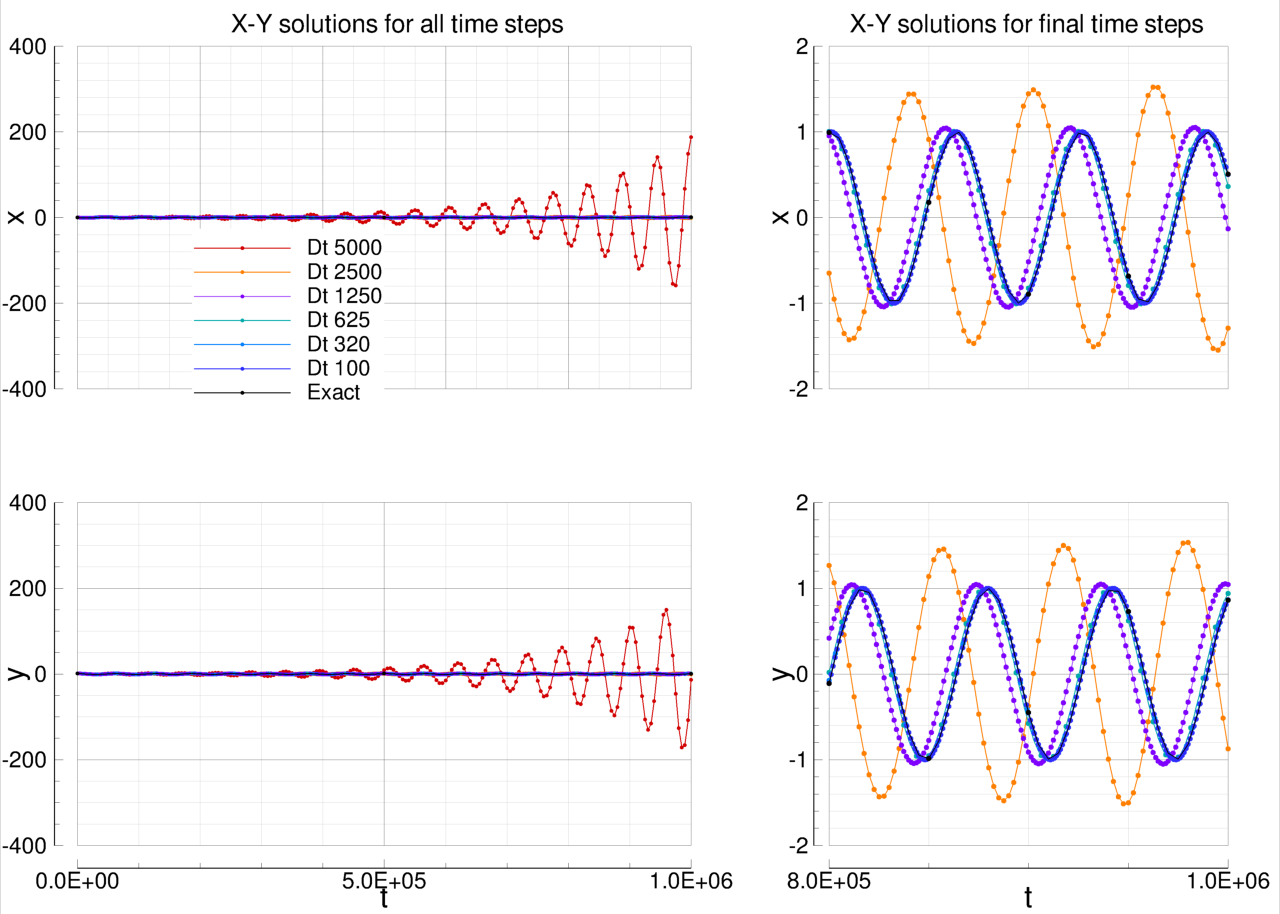
\includegraphics[width=1.00\textwidth]{errors-analysis/oscillation/errors_analysis-oscillation-adams-bashforth-2.png}
    \caption{2 steps}\label{fig:results-oscillation-adams-bashforth-2}
  \end{subfigure}\\
  \begin{subfigure}[b]{0.45\textwidth}
    \centering
    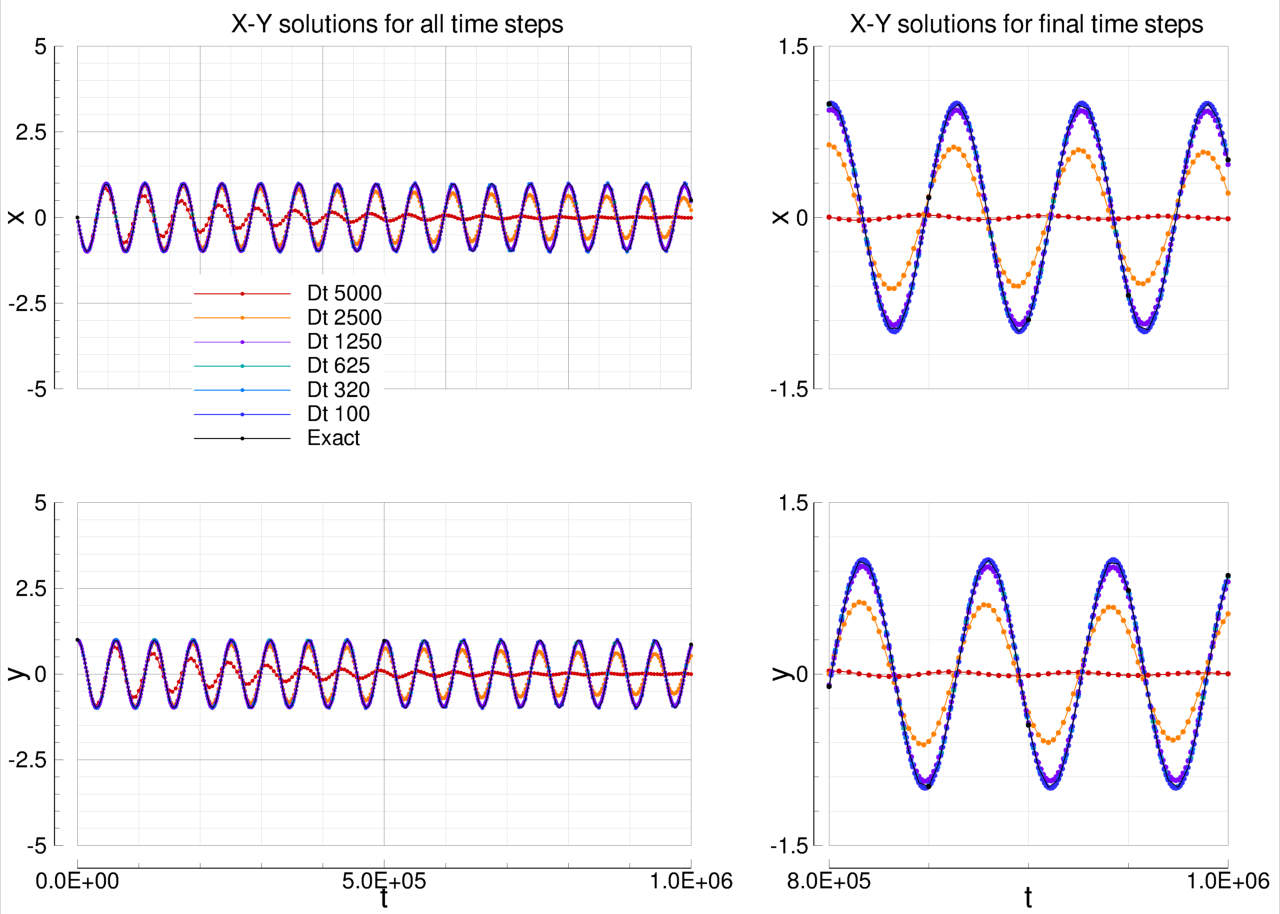
\includegraphics[width=1.00\textwidth]{errors-analysis/oscillation/errors_analysis-oscillation-adams-bashforth-3.png}
    \caption{3 steps}\label{fig:results-oscillation-adams-bashforth-3}
  \end{subfigure}\quad%
  \begin{subfigure}[b]{0.45\textwidth}
    \centering
    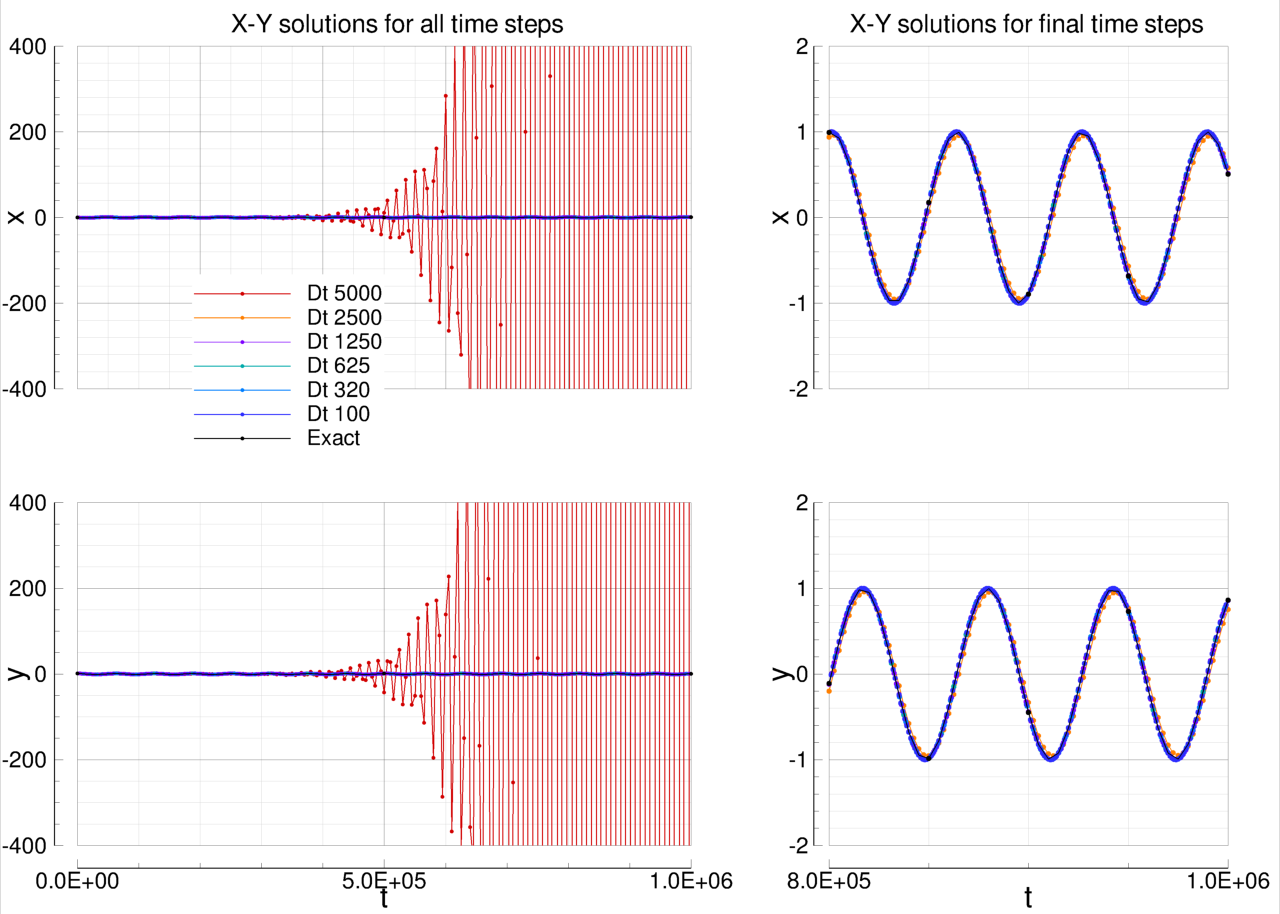
\includegraphics[width=1.00\textwidth]{errors-analysis/oscillation/errors_analysis-oscillation-adams-bashforth-4.png}
    \caption{4 steps}\label{fig:results-oscillation-adams-bashforth-4}
  \end{subfigure}
  \caption{Oscillation equations solutions computed by means of Adams-Bashforth solvers}\label{fig:results-oscillation-adams-bashforth}
\end{figure}

